\chapter{Spinning Switches}
\label{cha:research_topic_1}

TODO (Abstract)

\begin{enumerate}
  \item Generalizes switches to arbitrary groups.
  \item Proves a result when switches look like $p$-groups.
  \item Finds the ``correct'' model: the wreath products.
  \item Provides reductions for when strategies don't exist, which are easy to prove with the wreath product model.
  \item Comes up with an example where something isn't a prime power. ($S_3 \wr C_2$ is nontrivial. Of course $G \wr \mathbf{1}$ also works.)
\end{enumerate}

\section{TODO}
\begin{enumerate}
  \item Fill out Example \ref{ex:NoSolutionZ2C3}.
  \item Provide example for first reduction. (Theorem \ref{thm:SwitchReduction})
  \item Give other part of example for second reduction. (Theorem \ref{thm:SpinReduction})
  \item Example for third reduction. (Theorem \ref{thm:SpinReduction2})
  \item Define/discuss minimal switching strategies?
  \item Mention conjecture that most groups are $2$-groups
  \item Infinite switching strategy?
    $\mathbb{Z} \wr C_2$ or $\mathbb{Z}_2^\infty \wr C_2$. \\
    (By $\mathbb{Z}_2^\infty$, I mean something isomorphic to the integers under
    XOR: $(\mathbb{Z}, \oplus)$.)
\end{enumerate}

\section{Overview and Preliminaries}
This section provides a brief history of the problem and provides the idea for the more general context.
Section \ref{sec:WreathModel} models these generalizations in the context of the wreath product.
Section \ref{sec:HistoricalProgress} is where all of the references are. [TODO: put this section elsewhere]
Section \ref{sec:Reductions} allows us to prove when Player B does not have a winning strategy.
Section \ref{sec:pGroupStrategy} allows us to make a statement about games that have a prime number of possible moves.
Section \ref{sec:OtherSwitchingStrategies} gives us an example of new kinds of puzzles that have solutions.
Section \ref{sec:OpenQuestions} gives us an example of new kinds of puzzles that have solutions.

\subsection{History}
A closely related puzzle was popularized by Martin Gardner in the
February 1979 edition of his column ``Mathematical Games.'' \cite{Gardner1979Problem}
He wrote that he learned of the puzzle from Robert Tappay of Toronto who
``believes it comes from the U.S.S.R.''

The version under consideration in this paper is first hinted at in 1993
by Yehuda and collaborators \cite{Yehuda1993}.
Ehrenborg and Skinner consider something very similar, which they call the
"Blind Bartender with Boxing Gloves" \cite{Ehrenborg1995}.
This was re-popularized in 2019 when it appeared in ``The Riddler'' from
FiveThirtyEight \cite{FiveThirtyEight}.
Sidana \cite{Sidana2020} provides a detailed overview of the history of this
and related problems.

My preferred version appears in Peter Winkler's 2004 book
\textit{Mathematical Puzzles A Connoisseur's Collection}
\begin{quote}
  Four identical, unlabeled switches are wired in series to a light bulb.
  The switches are simple buttons whose state cannot be directly observed,
  but can be changed by pushing; they are mounted on the corners of a
  rotatable square. At any point, you may push, simultaneously, any subset
  of the buttons, but then an adversary spins the square. Show that there
  is a deterministic algorithm that will enable you to turn on the bulb in
  at most some fixed number of steps. \cite{Winkler2004}
\end{quote}

This version will be a working example in many parts of the paper, so it is
worth keeping in mind.

\subsection{A Solution to the Original Spinning Switches Puzzle}

In this short section, we will discuss the solution to this puzzle because it
will give some insights and intuition for the techniques that we use later.
It is useful to start with even a simpler example, which would make Peter
Winkler proud.

\begin{example}
  Suppose that instead of having four identical unlabeled switches, we instead
  only have two: on the diagonals of a rotatable square table.

  Then we have a three-step solution for solving the problem. We start by
  toggling both switches simultaneously. If this does not turn on the light,
  this means that the switches were (and still) are in different states.

  Then, the adversary spins the table. Next, we toggle one of the two switches
  to ensure that the switches are both in the same state. If the light hasn't
  turned on, both must be in the off state.

  The adversary spins the table once more, but to no avail. We know both
  switches are in the off state, so we toggle them both simultaneously, turning
  on the lightbulb.
\end{example}

In order to bootstrap this solution into a large solution, we must notice two
things.

First, if we can get two switches along each diagonal into the same state
respectively, then we can solve the puzzle by toggling both diagonals
(all four switches), both switches in a single diagonal, and both diagonals
again. In this (sub-)strategy, toggling both switches along a diagonal is
equivalent to toggling a single single switch in the above example.

Second, we can indeed get both diagonals into the same state by toggling a
switch from each diagonal (two switches on any side of square),
then a single switch from one diagonal,
followed by a switch from each switch.

We will interleave these strategies in a particular way, following the notation
of \cite{Rabinovich2022}.

\begin{definition}
  Given two sequences $A = \{a_i\}_{i=1}^N$ and $B = \{b_i\}_{i=1}^M$, we can
  define the \textbf{interleave} operation as \[
    A \circledast B = (
      \underbrace{a_1, a_2, \dots, a_N}_A,
      b_1,
      \underbrace{a_1, a_2, \dots, a_N}_A,
      b_2,
      \underbrace{a_1, a_2, \dots, a_N}_A,
      \dots,
      b_M,
      \underbrace{a_1, a_2, \dots, a_N}_A).
  \] which has length $(M+1)N + M = (M+1)(N+1)-1$.
\end{definition}

Typically it is useful to interleave two strategies when
$A$ solves the puzzle given that the switches are in a particular state, and
$B$ gets the switches into that particular state.
Usually, we also need $A$ not to ``interrupt'' what $B$ is doing.
In the problem of switches on a square table,
$B$ will ensure that the switches are in the same state within each diagonal,
and $A$ will turn on the light when that's the case.
Moreover, $A$ does not change the state within each diagonal.

\begin{proposition}
  There exists a fifteen-move strategy that guarantees that the light in
  Winkler's puzzle turns on.
\end{proposition}
\begin{proof}
  We begin by formalizing the two strategies. We will say that the first
  strategy $S_1$ where we toggle the two switches in a diagonal together
  will consist of the following three moves: \begin{enumerate}
    \item Switch \textbf{a}ll of the bulbs ($A$).
    \item Switch the \textbf{d}iagonal consisting of the upper-left and lower-right bulbs ($D$).
    \item Switch \textbf{a}ll of the bulbs ($A$).
  \end{enumerate}
  We will say that the second strategy $S_2$ where we get the two switches
  within each diagonal into the same state consists of the following three
  moves: \begin{enumerate}
    \item Switch both switches on the left \textbf{s}ide ($S$).
    \item Switch \textbf{one} switch ($1$).
    \item Switch both switches on the left \textbf{s}ide ($S$).
  \end{enumerate}
  Then the $15$ move strategy is \[
    S_1 \circledast S_2 = (A, S, A, D, A, S, A, 1, A, S, A, D, A, S, A)
  \]
\end{proof}

We will generalize this construct in
Theorem \ref{thm:switchingStrategyDecomposition},
which offers a formal proof that this strategy works.

It is worth briefly noting that $S_1 \circledast S_2$ is the fourth
\textit{Zimin word} (also called a \textit{sequipower}),
an idea that comes up in the study of combinatorics on words.

\subsection{Generalizing Switches}
``The problem can also be generalized by replacing glasses with objects that
have more than two positions. Hence the rotating table leads into deep
combinatorial questions that as far as I know have not yet been explored.''
\cite{Gardner1979Solution}

Two kinds of switches are considered by Yehuda, Etzionn, and Moran in 1993
\cite{Yehuda1993}: switches with a single ``on'' position that behave like
$n$-state roulettes ($\mathbb Z_n$) and switches that behave like
the finite field $\mathbb F_q$.
Yuri Rabinovich \cite{Rabinovich2022} goes further by considering collections
of switches that behave like arbitrary finite dimensional vector spaces over
finite fields.
We can generalize this notion further by considering
switches that behave like arbitrary finite groups.

\begin{example}
One could imagine a switch that behaves like the symmetric
group $S_3$, consisting of three identical-looking parts that need to be
arranged in a particular order in order for the switch to be on,
as illustrated in Figure \ref{fig:S3Switch}.
\end{example}

\begin{figure}
  \center{
  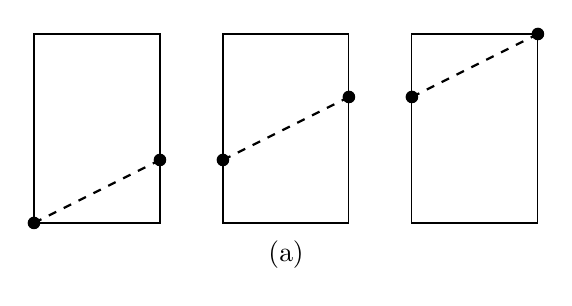
\begin{tikzpicture}[scale=0.8]
    \draw (0,0) rectangle ++(2,3);
    \draw[dashed,thick] (0,0) -- ++(2,1);
    \fill (0,0) circle (0.1);
    \fill (2,1) circle (0.1);

    \draw (3,0) rectangle ++(2,3);
    \draw[dashed,thick] (3,1) -- ++(2,1);
    \fill (3,1) circle (0.1);
    \fill (5,2) circle (0.1);

    \draw (6,0) rectangle ++(2,3);
    \draw[dashed,thick] (6,2) -- ++(2,1);
    \fill (6,2) circle (0.1);
    \fill (8,3) circle (0.1);
    \node at (4, -1/2) {(a)};
  \end{tikzpicture}
  }

  \noindent
  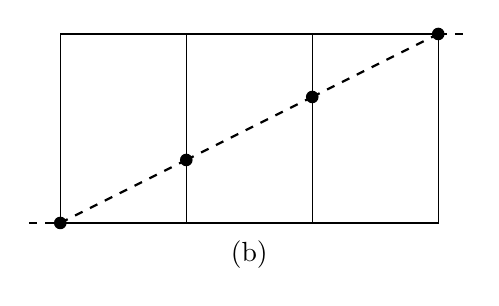
\begin{tikzpicture}[scale=0.8]
    \draw[dashed,thick] (-0.5,0) -- (0,0);
    \fill (0,0) circle (0.1);

    \draw (0,0) rectangle ++(2,3);
    \draw[dashed,thick] (0,0) -- ++(2,1);
    \fill (2,1) circle (0.1);

    \draw (2,0) rectangle ++(2,3);
    \draw[dashed,thick] (2,1) -- ++(2,1);
    \fill (4,2) circle (0.1);

    \draw (4,0) rectangle ++(2,3);
    \draw[dashed,thick] (4,2) -- ++(2,1);
    \fill (6,3) circle (0.1);

    \draw[dashed,thick] (6,3) -- (6.5,3);
    \node at (3, -1/2) {(b)};
  \end{tikzpicture}
  ~
  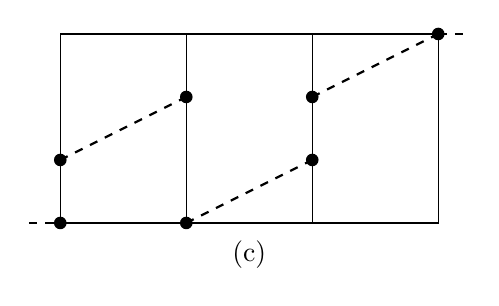
\begin{tikzpicture}[scale=0.8]
    \draw[dashed,thick] (-0.5,0) -- (0,0);
    \fill (0,0) circle (0.1);

    \draw (0,0) rectangle ++(2,3);
    \draw[dashed,thick] (0,1) -- ++(2,1);
    \fill (0,1) circle (0.1);
    \fill (2,2) circle (0.1);

    \draw (2,0) rectangle ++(2,3);
    \draw[dashed,thick] (2,0) -- ++(2,1);
    \fill (2,0) circle (0.1);
    \fill (4,1) circle (0.1);

    \draw (4,0) rectangle ++(2,3);
    \draw[dashed,thick] (4,2) -- ++(2,1);
    \fill (4,2) circle (0.1);
    \fill (6,3) circle (0.1);

    \draw[dashed,thick] (6,3) -- (6.5,3);
    \node at (3, -1/2) {(c)};
  \end{tikzpicture}
  \caption{
    Part (a) shows a simple schematic for a switch that behaves like $S_3$,
    the symmetric group on three letters.
    The three rectangles can be permuted arbitrarily, but only configuration (b)
    completes the circuit. All other configurations fail to
    complete the circuit (e.g. (c)).
  }
  \label{fig:S3Switch}
  \end{figure}

One subtlety is that we will use a group $G$ to model both the ``internal state''
of a switch itself and the set of ``moves'' or changes that can be made to the
switch. We can think of the moves changing the state via a right group action of
$G$ on itself.

The reason that using a group to model a switch is because groups have many
of the properties we would expect in a desirable switch.
\begin{note}
  The group axioms for a group $(G, \cdot)$ are
\end{note}
 \begin{enumerate}
  \item (Closure) The group $(G, \cdot)$ is equipped with a binary operation,
  $\cdot \colon G \times G \rightarrow G$. That is, for all pairs of elements
   $g_1, g_2 \in G$ their product is in $G$ \[
     g_1 \cdot g_2 \in G.
  \]
  In the context of switches, this
  means that if the switch is in some state $g_1 \in G$ and player B moves
  it with action $g_2 \in G$, then $g_1 \cdot g_2 \in G$ is a valid switch for
  the state.
  %
  %
  \item (Identity) There exists an element $\operatorname{id}_G \in G$ such that
  for all $g \in G$, \[
    \operatorname{id}_G \cdot g = g \cdot \operatorname{id}_G = g.
  \]
  This axiom is useful because it means that Player B can ``do nothing''
  to a switch and leave it in whatever state it is in.
  Because the identity is a distinguished element in $G$,
  we will also use the convention that
  $\operatorname{id}_G$ is the ``on'' or ``winning'' state for a given switch.
  (It is worth noting that all of the arguments work with small modification
  regardless of which element is designated as the on state.)
  %
  %
  \item (Inverses) For each element $g \in G$ there exists an inverse element
  $g^{-1} \in G$ such that \[
    g \cdot g^{-1} = g^{-1} \cdot g = \operatorname{id}_G.
  \]
  This axiom states that no matter what state a switch is in,
  there is a move that will transition it into the on state.
  %
  %
  \item (Associativity) Given three elements $g_1, g_2, g_3 \in G$,
  \[
    (g_1 \cdot g_2) \cdot g_3 = g_1 \cdot (g_2 \cdot g_3)
  \]
  This is axiom is not strictly necessary for modeling switches,
  but as we will see in a later definition, it gives us a convenient way to
  describe the conditions for a winning strategy.
  (In Subsection \ref{sub:quasigroupSwitches}, we briefly discuss dropping
  the associativity axiom by considering switches that behave like
  quasigroups with identity.)
\end{enumerate}

% In a similar vein, we could construct a switch that behaves like the dihedral
% group of the square. Perhaps the switch is a thin square prism that fits into a
% square slot in such a way that only one orientation of the prism completes the
% circuit. See Figure \ref{fig:D8Switch} for a simple schematic.
% [A schematic for a switch that looks like $D_4$.]
% Or one could imagine a switch that behaves like the dihedral group of the square,
% $D_8$ where the square has a single, unique orientation that completes the circuit.
% Or abstractly, one could think of each switch as an abstract group element,
% where Player B can multiply by anything they like.

\subsection{Generalizing Spinning}
We can also consider generalizations of ``spinning'' the switches.
In particular, we will adopt the generalization from
Ehrenborg and Skinner's \cite{Ehrenborg1995} 1995 paper, which use
arbitrary finite group actions to permute the switches.
In particular, they provide a criterion that determines which group actions
yield a winning strategy in the case of a given number of ``ordinary'' switches
(those that behave like $\mathbb Z_2$).
Rabinovich \cite{Rabinovich2022} stretches these results a bit further and
looks at certain group actions on collections of switches that behave like
a finite dimensional vector space over a finite field. We build on this result
in the context of more general switches.

\section{The Wreath Product Model}
\label{sec:WreathModel}
Peter Winkler's version of the puzzle consists of four two-way switches on the
corners of a rotating square table.
The behavior of the switches are naturally modeled as $\mathbb Z_2$, and
the rotating table is modeled as the cyclic group $C_4$.

If we put these together as a wreath product of $\mathbb Z_2$ by $C_4$, it
will result in the expected structure.
\subsection{Modeling Generalized Spinning Switches Puzzles}
\begin{definition}[\cite{Rotman1999}]
  Let $G$ and $H$ be groups,
  let $\Omega$ be a finite $H$-set, and
  let $K = \prod_{\omega \in \Omega} G_\omega$, where $G_\omega \cong G$
  for all $\omega \in \Omega$.
  Then the \textbf{wreath product} of $G$ by $H$ denoted by $G \wr H$,
  is the semidirect product of $K$ by $H$,
  where $H$ acts on $K$ by $h \cdot (d_\omega) = d_{h^{-1}\omega}$ for $g \in H$ and
  $(g_\omega) \in \prod_{\omega \in \Omega} G_\omega$.
  The normal subgroup $K$ of $G \wr H$ is called
  the \textbf{base} of the wreath product.

  The group operation is $(k, h) \cdot (k', h') = (k(h \cdot k'), hh')$j
\end{definition}

The reason this definition is used is because it models the game well:
$G$ models the behavior of the switches, $\Omega$ models the positions of the
switches, and the action of $H$ on $\Omega$ models the ways the adversary can
``spin'' or scramble the switches.

An element of $(k, h) \in G \wr H$ represents a turn of the game:
Player B chooses an element of the base $k \in K$ to indicate
how they want to modify each of their switches
and then Player A chooses $h \in H$ to indicate how they want to permute the
switches.

\begin{example}
  Consider the setup in the original version of the problem consisting of
  two-way switches ($\mathbb Z_2$)
  on the corners of a rotating square
  ($C_4 \cong \langle 0^\circ, 90^\circ, 180^\circ, 270^\circ \rangle$).
  This can be modeled as a game on the wreath product $\mathbb Z_2 \wr C_4$.
  We will use the convention that the base of the wreath product, $K$ is
  ordered upper-left, upper-right, lower-right, lower-left, and the group
  action is specified by degrees in the clockwise direction.

  Consider the following two turns:
  \begin{enumerate}
    \item During the first turn,
    Player B toggles the upper-left and lower-right switches, and
    Player A rotates the table $90^\circ$ clockwise.
    This is represented by the element
    $((1,0,1,0), 90^\circ) \in \mathbb Z_2 \wr C_4$.
    \item During the second turn,
    Player B toggles the upper-left switch, and
    Player A rotates the table $90^\circ$ clockwise.
    This is represented by the element
    $((1,0,0,0), 180^\circ) \in \mathbb Z_2 \wr C_4$.
  \end{enumerate}
  %
  As illustrated in Figure \ref{fig:WreathProduct},
  the net result of these two turns is the same as
  a single turn where Player B toggles the upper-left, upper-right, and lower-left
  switches and Player A rotates the board $270^\circ$ clockwise.

  \begin{figure}
    \center
    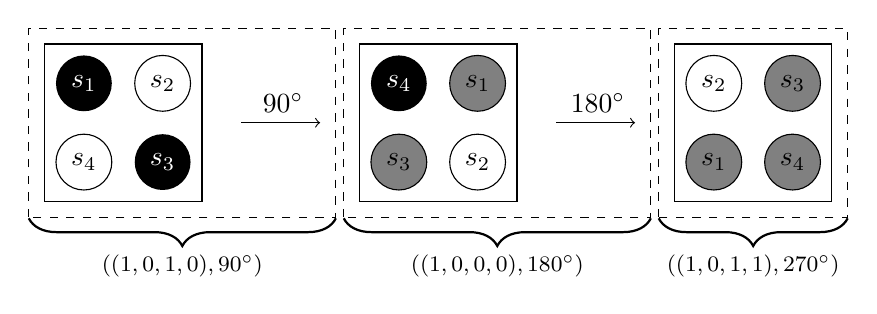
\begin{tikzpicture}
      \draw[dashed] (-0.2,-0.2) rectangle (3.7,2.2);
      \draw [thick,decorate,decoration={brace,amplitude=10pt},yshift=-0.4pt]
        (3.7,-0.2) -- (-0.2,-0.2) node[black,midway,yshift=-0.6cm] {\footnotesize $((1,0,1,0), 90^\circ)$};

      \draw[dashed] (3.8,-0.2) rectangle (7.7,2.2);
      \draw [thick,decorate,decoration={brace,amplitude=10pt},yshift=-0.4pt]
        (7.7,-0.2) -- (3.8,-0.2) node[black,midway,yshift=-0.6cm] {\footnotesize $((1,0,0,0), 180^\circ)$};

      \draw[dashed] (7.8,-0.2) rectangle (10.2,2.2);
      \draw [thick,decorate,decoration={brace,amplitude=10pt},yshift=-0.4pt]
        (10.2,-0.2) -- (7.8,-0.2) node[black,midway,yshift=-0.6cm] {\footnotesize $((1,0,1,1), 270^\circ)$};

      \draw (0,0) rectangle (2,2);
      \node[circle,fill,text=white] at (1/2,3/2) {$s_1$};
      \node[circle,draw] at (3/2,3/2) {$s_2$};
      \node[circle,fill,text=white] at (3/2,1/2) {$s_3$};
      \node[circle,draw] at (1/2,1/2) {$s_4$};
      \draw[->] (2.5,1) -- node[above] {$90^\circ \! \curvearrowright$} (3.5,1) ;

      \draw (4,0) rectangle (6,2);
      \node[circle,fill,text=white] at (9/2,3/2) {$s_4$};
      \node[circle,draw,fill=gray] at (11/2,3/2) {$s_1$};
      \node[circle,draw] at (11/2,1/2) {$s_2$};
      \node[circle,draw,fill=gray] at (9/2,1/2) {$s_3$};

      \draw[->] (6.5,1) -- node[above] {$180^\circ \! \curvearrowright$} (7.5,1) ;

      \draw (8,0) rectangle (10,2);
      \node[circle,draw] at (17/2,3/2) {$s_2$};
      \node[circle,draw,fill=gray] at (19/2,3/2) {$s_3$};
      \node[circle,draw,fill=gray] at (19/2,1/2) {$s_4$};
      \node[circle,draw,fill=gray] at (17/2,1/2) {$s_1$};
    \end{tikzpicture}
    \caption{An illustration of two turns each in the Spinning Switches puzzle,
    modeled as elements of a wreath product.}
    \label{fig:WreathProduct}
  \end{figure}

  The multiplication under the wreath product agrees with this: \begin{align*}
    ((1,0,1,0), 90^\circ) \cdot ((1,0,0,0), 180^\circ)
    &= ((1,0,1,0) + \underbrace{90^\circ \cdot (1,0,0,0)}_{(0,0,0,1)}, 90^\circ + 180^\circ) \\
    &= ((1,0,1,1), 270^\circ)
  \end{align*}
\end{example}

Occasionally it is useful to designate a particular state of the switches as the
on state or the winning state, and ordinarily the identity state is the choice
given for this. However, the existence of a winning strategy does not depend on
a particular choice in the winning state; instead, a winning strategy is
equivalent to a choice of moves that will walk over all of the possible
configuration states, regardless of the choice of the adversaries spin.

\subsection{Switching Strategy}

\begin{definition}
  A \textbf{switching strategy} is a finite sequence, $\{k_i \in K\}_{i=1}^N$,
  such that for every sequence ${\{h_i \in H\}_{i=1}^N}$,
  \[
    p(\{
      \underbrace{e_{G \wr H}}_{m_0},
      \underbrace{(k_1, h_1)}_{m_1},
      \underbrace{(k_1, h_1)\cdot(k_2, h_2)}_{m_2},
      \cdots,
      \underbrace{(k_1, h_1)\cdot(k_2, h_2)\cdots(k_N, h_N)}_{m_N}
    \}) = K.
  \]
  where $p \colon G \wr H \rightarrow K$ is the projection map from the
  wreath product onto its base.
\end{definition}

This definition is useful because it puts the problem into purely algebraic
terms. It is also useful because it abstracts away the initial state of the
switches: regardless of the initial state $k \in K$, a existence of a switching strategy
means that its inverse $k^{-1} \in K$ appears in the sequence.

% This abstracts away the notion of which $k \in K$ represents the ``on'' state,
% although it is natural to choose $\operatorname{id}_k \in K$ to play this role.

\begin{lemma}
  A sequence of moves is guaranteed to ``turn on the lightbulb'' if and only if
  it is a switching strategy.
\end{lemma}
\begin{proof}
  Without loss of generality, say that the ``on'' setting for the switches is
  $\mathrm{id}_K$.
  In the puzzle, we have an initial (hidden) state, $k$.
  Thus, after the $i$-th move, the wreath product
  element that represents the state of the switches is \[
    p\left((k, \mathrm{id}_H)\cdot(k_1, h_1)\cdot(k_2, h_2)\cdots(k_i, h_i)\right)
    = k \cdot p\left((k_1, h_1)\cdot(k_2, h_2)\cdots(k_i, h_i)\right),
  \] by associativity, where we can factor out the first term because
  the ``spin'' is $\mathrm{id}_H$, which acts trivially, that is
  $(k, \mathrm{id}_H) \cdot (k', h') = (kk', h').$

  Thus, by considering different initial states, we see that in order
  to reach the on state, there must exist some $i$, such that
  $p\left((k_1, h_1)\cdot(k_2, h_2)\cdots(k_i, h_i)\right) = k^{-1}$ for all
  $k$ and adversarial sequences $\{h_i\}_{i=1}^N$.
\end{proof}

It's also worth noting that this model can be thought of as a random model or an
adversarial model: the sequence $\{h_i \in H\}$ can be chosen after the sequence
$\{k_i \in K\}$ in a deterministic way or randomly.

One useful consequence of this definition is that it quite straightforward to
prove certain lemmas. For example, the minimum length for a switching strategy
has a simple lower bound.
\begin{lemma}
  Every switching strategy $\{k_i \in K\}_{i=1}^{N}$ is a sequence of
  length at least $|K| - 1$.
\end{lemma}
\begin{proof}
  By the pigeonhole principle, because the set \[
    \{e_{G \wr H}, (k_1, h_1), (k_1, h_1)\cdot(k_2, h_2), \cdots, (k_1, h_1)\cdot(k_2, h_2)\cdots(k_N, h_N)\}
  \] has at most $N+1$ elements. In order for the projection to be equal to $K$, \[
    p(\{e_{G \wr H}, (k_1, h_1), (k_1, h_1)\cdot(k_2, h_2), \cdots, (k_1, h_1)\cdot(k_2, h_2)\cdots(k_N, h_N)\}) = K,
  \] $N+1 \geq |K|$, so $N \geq |K| - 1$.
\end{proof}

\begin{definition}
  A \textbf{minimal switching strategy} for $G \wr H$ is a switching strategy
  of length $N = |K| - 1.$
\end{definition}

In practice, every wreath product known by the author to have a switching
strategy also has a known minimal switching strategy.
In Section \ref{sec:OpenQuestions}, we ask whether this property always holds.

% TODO: Is it worthwhile to mention that
% variants of this puzzle require more constraints---
% if you can only change $k$ switches,
% or if all of the switches need only to be in the same state,
% or if you can see the states of the switches and player A rotates after you specify what you want.

\section{Reductions}
\label{sec:Reductions}
There are essentially three ways to show that $G \wr H$ does not have a
solution: directly, or via one of two \textit{reductions} (or a combination thereof).

\subsection{Puzzles Without Switching Strategies}
Using results from Rabinovich \cite{Rabinovich2022}, we can give examples of
puzzles that don't have solutions. This section allows us to take those examples
and stretch them into wider families of examples.

\begin{example}
  % Yehuda's ``open game'' makes it clear that $\mathbb Z_2 \wr C_3$ doesn't have a strategy.
  The game $\mathbb Z_2 \wr C_3$ does not have a switching strategy. Here's how to see it...
  \label{ex:NoSolutionZ2C3}
\end{example}

\subsection{Reductions on Switches}
\begin{theorem}
  If $G \wr H$ does not have a switching strategy and $G'$ is a group with
  a quotient $G'/N \cong G$, then ${G'} \wr H$ does not have a switching
  strategy.
  \label{thm:SwitchReduction}
\end{theorem}
\begin{proof}
  I will prove the contrapositive, and suppose that $G' \wr H$ has a
  switching strategy $\{k'_i \in K'\}_{i=1}^N$. The quotient map
  $\varphi\colon G' \mapsto G$
  extends coordinatewise to
  $\hat\varphi \colon K' \mapsto K$.

  The sequence $\{\hat\varphi(k'_i) \in K\}_{i=1}^N$ is a switching strategy on
  $G \wr H$.
  [Say something about how the projection map is ?linear? wrt $\hat\varphi$?
  Say $\phi$ induces a homomorphism from $G' \wr H$?]

  Want to prove \[
    p((\hat\varphi(k'_1),h_1)\dots(\hat\varphi(k'_i),h_i)) =
    \hat\varphi(p'((k'_1,h_1)\dots(k'_i,h_i)))
  \] where $p \colon G \wr H \rightarrow K$ and $p' \colon G' \wr H \rightarrow K'$
\end{proof}
\begin{example}
  We know that $\mathbb Z_2 \wr C_3$ doesn't have a switching strategy.
  This means that $\mathbb Z_6 \wr C_3$ does not have a switching strategy either.
  This is illustrated in Figure \ref{fig:Z2C3}
  \begin{figure}
    \center
    \includegraphics{assets/tikz_Z2C3.pdf}
    \caption{
      A reduction on switches:
      $\mathbb Z_6 \wr C_3$ reduces to $\mathbb Z_2 \wr C_3$,
      which is known not to have a switching strategy.
    }
    \label{fig:Z2C3}
  \end{figure}
\end{example}
\subsection{Reductions on Spinning}
\begin{theorem}
  If $G \wr H$ does not have a switching strategy and $H'$ is a group with
  a subgroup $A \leq H'$ such that $A \cong H$, then
  $G \wr H'$ does not have a switching strategy.
  \label{thm:SpinReduction}
\end{theorem}
\begin{proof}
  Again we will prove the contrapositive.
  Assume that $G \wr H'$ does have a switching strategy,
  $\{k_i\}_{i=1}^N$. Then by definition, for any sequence
  $\{h'_i\}_{i=1}^N$, the projection of the sequence \[
    p(\{(k_1, h'_1)\cdot(k_2, h'_2)\cdots(k_i, h'_i)\}_{i=1}^N) = K,
  \] and in particular this is true when $h'_i$ is restricted to be in the
  subgroup $H$. Thus a switching strategy for $G \wr H'$ is also a valid
  switching strategy for $G \wr H$.
\end{proof}

\begin{example}
  We know that $\mathbb Z_2 \wr C_3$ doesn't have a switching strategy.
  This means that $\mathbb Z_2 \wr C_6$ does not have a switching strategy either.
  \begin{figure}
    \center
    \includegraphics{assets/tikz_Z2C6.pdf}
    \caption{If there were a solution to $\mathbb Z_2 \wr C_6$, then there
    would be a solution to ...}
  \end{figure}
\end{example}

(TODO: commentary: What we're more interested in though is the reduction of
$\mathbb Z_2 \wr C_6$ to $\mathbb Z_2 \wr C_3$.
(Closely related to Theorem \ref{thm:SpinReduction})
)
\begin{theorem}
  Suppose that $H'$ is a group with a subgroup $A \leq H'$ such that
  $A \cong H$,
  and let \[
    \operatorname{Orb}(\omega) = \{\omega \cdot a : a \in A \} \subseteq \Omega
  \]
  be the (right) orbit of $\omega \in \Omega$ under $A$.
  If $G \wr_{\operatorname{Orb}(\omega)} H$ does not have a switching strategy,
  then $G \wr_\Omega H'$ does not have a switching strategy.
  \label{thm:SpinReduction2}
\end{theorem}
\begin{proof}
  We start by making the contrapositive assumption that $G \wr_\Omega H'$
  has a switching strategy $\{k_i \in K\}_{i=1}^N$, and we consider the projection
  $p_\omega \colon K \rightarrow K_\omega$ where
  $K = \prod_{\omega \in \Omega} G_\omega$ and
  $K_{\omega} = \prod_{\omega' \in \operatorname{Orb}(\omega)} G_{\omega'}$.

  Then $\{p_\omega(k_i) \in K_\omega\}_{i=1}^N$ is a switching strategy for
  $G \wr_{\operatorname{Orb}(\omega)} H$, since a projection is a surjective
  map.
\end{proof}

\begin{example}
  We know that $\mathbb Z_2 \wr C_3$ doesn't have a switching strategy.
  This means that $\mathbb Z_2 \wr C_6$ does not have a switching strategy either.
  \begin{figure}
    \center
    \includegraphics{assets/tikz_Z2C6_2.pdf}
    \caption{We know that $\mathbb Z_2 \wr_\Omega C_6$ cannot have
    a switching strategy, because that would imply a switching strategy for
    $\mathbb Z_2 \wr_{\Omega'} C_3$, where $\Omega'$
    is the orbit of the top switch rotations of multiples of $120^\circ$.}
  \end{figure}
\end{example}

%%%%%%%%%%%%%%%%%%%%%%%%%%%%%%%%%%%%%%%%%%%%%%%%%%%%%%%%%%%%%%%%%%%%%%%%%%%%%%
%
% Switching strategies on p-groups
%
%%%%%%%%%%%%%%%%%%%%%%%%%%%%%%%%%%%%%%%%%%%%%%%%%%%%%%%%%%%%%%%%%%%%%%%%%%%%%%
\section{Switching Strategies on \texorpdfstring{$p$}{p}-Groups}
\label{sec:pGroupStrategy}
In this section, we'll develop a broad family of switching strategies,
namely those on $p$-groups.
\subsection{Switching Strategy Decomposition}

% TODO: introduce the interweave operator, motivated by an example.

Our first constructive theorem provides a technique that can be used to
construct switching strategies for switches that behave like a group $G$ in
terms of a normal group and its corresponding quotient group.
\begin{theorem}
  The wreath product $G \wr H$ has a switching strategy if there exists a
  normal subgroup $N \trianglelefteq G$ such that both $N \wr H$ and
  $G/N \wr H$ have switching strategies.
\label{thm:switchingStrategyDecomposition}
\end{theorem}
\begin{proof}
  Let $S_{G/N} = \{k_i^{G/N} \in K_{G/N}\}$ denote the switching strategy for $G/N \wr H$, and
  let $S_{N} = \{k_i^N \in K_{N}\}$ denote the switching strategy for $N \wr H$.

  First, we partition $G$ into $|G|/|N| = m$ cosets of $N$: \[
    G = g_1N \sqcup g_2N \sqcup \dots \sqcup g_mN.
  \]

  From the switching strategy $\{k_i^{G/N} \in K_{G/N}\}$,
  we can get a sequence $S_{G'} = \{k_i' \in K_G\}$
  by picking the coset representatives coordinatewise.

  This sequence is not itself a switching strategy, but it does ``hit'' all
  combinations of cosets. That is, for every ``spinning sequence'' $\{h_i \in H\}$,
  and sequence of cosets $(g_{i_1}H, g_{i_2}H, \dots, g_{i_m}H)$, there exists
  an index $n$ such that \[
    p((k_1', h_1) \dots (k_n', h_n)) \in g_{i_1}H \times g_{i_2}H \times \dots \times g_{i_m}H
  \]

  Now if we interleave $S_G' \circledast S_N$, this forms a
  switching strategy because ... \[
    S_G' \circledast S_N = (\underbrace{k^N_1, k^N_2, \dots, k^N_{n_N}}_{B_0}, \underbrace{k'_1, k^N_1, k^N_2, \dots, k^N_{n_N}}_{B_1}, \dots, \underbrace{k'_{n'}, k^N_1, k^N_2, \dots, k^N_{n_N}}_{B_{n'}})
  \]

  The partial products that end in block $B_i$ all have switches in the same
  cosets of $N$, and the $S_N$ strategy then hits all elements of $K_G$ that
  belong to that combination of cosets.

  % First, we choose representatives ${g_1, g_2, \dots, g_{m}}
\end{proof}
\begin{theorem} \cite{Rabinovich2022}
  Assume that a finite group $H$ acts linearly and faithfully on a vector space
  $V$ over a finite field $\mathbb F_q$ of characteristic $p$.
  Then $(G, V)$ is friendly if and only if $G$ is a $p-group$.
\end{theorem}
\begin{corollary}
  If $H$ is a finite group that acts faithfully on $\Omega$, then the wreath product
  $G \wr H$ has a switching strategy whenever $|G| = p^n$ for some $n$.
\end{corollary}
\begin{proof}
  If $|G| = p^n$, then either $G \cong \mathbb{Z}_p$ or $G$ is not simple.
  If $G \cong \mathbb{Z}_p$, then there exists a strategy. Otherwise,
  $G$ is not simple, so choose a normal subgroup $N$ of order $|N| = p^t$
  which gives a quotient $G/N$ with order $|G/N| = p^{n-t}$. Then the
  result follows by induction.
\end{proof}
\begin{corollary}
  Based on the above construction, if $|G| = p^n$, then $G \wr C_{p^\ell}$
  has a palindromic strategy of length $p^{n p^\ell}-1$.
\end{corollary}
\begin{proof}
  Is this true for general $H \neq C_{p^\ell}$?
\end{proof}

%%%%%%%%%%%%%%%%%%%%%%%%%%%%%%%%%%%%%%%%%%%%%%%%%%%%%%%%%%%%%%%%%%%%%%%%%%%%%%
%
% Switching strategies on permutations
%
%%%%%%%%%%%%%%%%%%%%%%%%%%%%%%%%%%%%%%%%%%%%%%%%%%%%%%%%%%%%%%%%%%%%%%%%%%%%%%
\section{Switching Strategies on Other Wreath Products}
\label{sec:OtherSwitchingStrategies}

So far, the literature has only contained examples of spinning strategies on
wreath products that are themselves $p$-groups:
$|G \wr_\Omega H| = |G|^{|\Omega|} \cdot |H|$, where $H$ acts faithfully.

\subsection{\texorpdfstring{$G \wr \mathbf{1}$}{The trivial wreath product}}

Of course, if $H = \textbf{1}$ is the trivial group, then
$G \wr \mathbf{1} \cong G$ has a switching strategy even if $G$ is not a $p$-group.
(In fact, it has $(|G|-1)!$ switching strategies!)

\subsection{Two interchangeable copies of a symmetric group \texorpdfstring{$S_n \wr C_2$}{Sn wr C2}}

\begin{theorem}
  $S_n \wr C_2$ has a switching strategy.
\end{theorem}

We'll construct a switching strategy.
Now our switching strategy has two parts: the first is that we ensure that
the two switches have every possible difference. The second is that we show
that we can get either of the switches to take on every possible value without
disturbing the difference.

\begin{proof}
  We start with the observation that the symmetric group can be generated by
  transpositions: $S_n = \langle t_1, t_2, \dots, t_N\rangle$.
  This means that there is a sequence of transpositions $t_{i_1}, t_{i_2}, \dots, t_{i_M}$
  such that $\{\mathrm{id}, t_{i_1}, t_{i_1}t_{i_2}, \dots, t_{i_1}t_{i_2}\cdots t_{i_M}\} = S_n$.

  Strategy A: We first assume that we have a sequence of moves that can run
  through all values of the first coordinate.
  Of course we do, just let $t' = (t, t) \in K$ and use the sequence
  $\{t'_{i_1}, t'_{i_2}, \dots , t'_{i_M}\}$.

  Strategy B: Let the $i$-th move be denoted by $m_i = (k_i, k_i')$.
  We want $t_1t_2^{-1}$ to be whatever we choose. We can do this too by
  applying the sequence $\{(t_{i_j}, \operatorname{id}_G)\}_{j=1}$ this is because
  \[
    t_1(t_2t)^{-1} = t_1t^{-1}t_2^{-1} = (t_1t)t_2^{-1}
  \] because $t$ is a transposition, and thus $t = t^{-1}$.
  Moreover, when we apply the first strategy, it doesn't change this difference:
  $(t_1t)(t_2t)^{-1} = t_1tt^{-1}t_2^{-1} = t_1t_2^{-1}$

  Combined: $S_2 \circledast S_1$
\end{proof}
\begin{example}
  If $a \in S_3$, let $a_1$ mean multiplying one of the two copies by $a$ and
  $a_2$ mean multiplying both of the copies by $a$. Then the following is
  a strategy:
  \begin{align*}
    (12)_2(13)_2(12)_2(13)_2(12)_2 \\
    &(12)_1 \\
    (12)_2(13)_2(12)_2(13)_2(12)_2 \\
    &(13)_1 \\
    (12)_2(13)_2(12)_2(13)_2(12)_2 \\
    &(12)_1 \\
    (12)_2(13)_2(12)_2(13)_2(12)_2 \\
    &(13)_1 \\
    (12)_2(13)_2(12)_2(13)_2(12)_2 \\
    &(12)_1 \\
    (12)_2(13)_2(12)_2(13)_2(12)_2
  \end{align*}
  \label{ex:TwoSymmetricGroups}
\end{example}
In general, if you can walk through $G$ with elements of order $2$, then
there is a strategy.
%%%%%%%%%%%%%%%%%%%%%%%%%%%%%%%%%%%%%%%%%%%%%%%%%%%%%%%%%%%%%%%%%%%%%%%%%%%%%%
%
% Open questions
%
%%%%%%%%%%%%%%%%%%%%%%%%%%%%%%%%%%%%%%%%%%%%%%%%%%%%%%%%%%%%%%%%%%%%%%%%%%%%%%
\section{Open questions}
\label{sec:OpenQuestions}
\subsection{Palindromic switching strategies}
In all known examples, when there exists a switching strategy $S$,
there exists a \textit{palindromic} switching strategy
$S' = \{k'_i \in K\}_{i=0}^N$
such that $k'_i = k'_{N-i}$ for all $i$.
\begin{conjecture}
  Whenever $G \wr H$ has a switching strategy, it also has a palindromic switching
  strategy.
\end{conjecture}

I'm interested in the answer even in the case of $G \wr \mathrm{1} \equiv G$.

(\href{https://math.stackexchange.com/q/3706654/121988}{MSE})

\subsection{Quasigroup switches}
\label{sub:quasigroupSwitches}
In the paper we modeled switches as groups.
This is because groups have desirable properties: \begin{enumerate}
  \item Closure. Regardless of which state a switch is in, modifying the state is the set of states.
  \item Identity. We don't have to toggle a switch on a given turn.
  \item Inverses. If a switch is off, we can always turn it on.
\end{enumerate}

It turns out that we don't need the axiom of associativity,
because the sequencing is naturally what computer scientists call
``left associative''. Thus, we can model switches a bit more generally as
\textit{loops} (i.e. quasigroups with identity.)

\subsection{Expected number of turns}
Recall that the original conception of a generalized spinning switches puzzle
is to turn on all of the switches at once. That if the original state of
the puzzle is $k \in K$,
we ``win'' on move $i$ if $k^{-1} = p((k_1, h_1)(k_2, h_2)\dots(k_i, h_i))$.
It is natural to ask about the expected value of the number of turns given
various sequences of moves. Notice that this is a question we can ask
even about generalized spinninng switches puzzles that do not have a switching
strategy.

Indeed, Winkler \cite{Winkler2004} (TODO, this is probably the wrong citation!)
notes in the solution of his puzzle:
\begin{quote}
  This puzzle reached me via Sasha Barg of the University of Maryland,
  but seems to be known in many places. Although no fixed number of steps
  can guarantee turning the bulb on in the three-switch version [with two-way switches],
  a smart randomized algorithm can get the bulb on in at most $5 \frac{5}{7}$
  steps on average, against any strategy by an adversary who sets the initial
  configuration and turns the platform. \cite{Winkler2021}
\end{quote}

% flip, guess, flip, guess, flip, guess, ...
%
% 1/7 & 1/6 & 1/5 &

% 1 * 1/7 +
% 2 * (6/7*1/6) +
% 3 * (6/7*5/6*1/5) +
% 4 * (6/7*5/6*4/5*1/6)
% ...
%
% = 1/7 + (6/7)*[
%   (2/6)*(1(2/3)^0 + 2(2^3)^1 + ...))
%   (1/6)*(3() + 5 + 7 + ...)
In all cases, when computing the expected number of turns, we will assume that
the initial hidden state $k \in K$ is not the winninng state $\mathrm{id}_K$,
and that the adversaries ``spins'' are indepedent and identically distributed
uniformly random elements $h_j \in H$.

\begin{proposition}
  If Player $B$ chooses $k_j \in K \setminus \{\mathrm{id}_K\}$ uniformly at random
  (that is, never choosing the ``do nothing'' move) then the distribution
  of the resulting state will be uniformly distrubuted among the $|K| - 1$
  different states, the probability of the resulting state being the
  winning state is
  \[
    \mathbb{P}(p((k_1, h_1)(k_2, h_2)\dots(k_j, h_j))=k^{-1}\ |\ p((k_1, h_1)(k_2, h_2)\dots(k_{j-1}, h_{j-1})\neq k^{-1})) = \frac{1}{|K| - 1},
  \] and the expected number of moves is $|K| - 1$.
\end{proposition}
\begin{proof}
  Because the new states are in $1$-to-$1$ correspondence with the elements of
  $K \setminus \{\mathrm{id}_K\}$, since $k_j \in \setminus \{\mathrm{id}_K\}$
  is chosen uniformly at random, $p((k_1, h_1)(k_2, h_2)\dots(k_j, h_j)$
  is uniformly distributed among all elements of $K$ besides the projection of
  the first $j-1$ elements.
  The expected value is $|K| - 1$ because the number of turns follows a
  geometric distribution with parameter $(|K| - 1)^{-1}$.
\end{proof}

Unsuprisingly, when a generalized spinning switches puzzle has a
\textit{minimal} switching strategy, then we can do better than this, on average.

\begin{proposition}
If the generalized spinning switches puzzle, $G \wr H$, has a minimal switching
strategy, then the expected number of moves is $|K|/2$.
TODO: And no other strategy can do better than this.
\end{proposition}
\begin{proof}
  TODO: Every move is equally likely to be our winner. (clean up proof)

  If there's a switching strategy of length $|K| - 1$,
  then the sequence walks through every state exactly once,
  and so every move is equally likely
  we're equally likely to win on any turn, so
  the expected number is $(N+1)/2$ with an $N$ move strategy.
\end{proof}

\begin{proposition}
  Whether or not the generalized spinning switches puzzle $G \wr H$ has
  a switching strategy, there always exists a (perhaps infinite) strategy
  whose expected value of moves is strictly less than $|K| - 1$.
\end{proposition}
\begin{proof}
  We can always do a bit better than the naive play by saying never do
  $(g,g, ..., g) \in K$ followed by $(g^{-1},g^{-1}, ..., g^{-1}) \in K$.
\end{proof}

\begin{conjecture}
  There exists a constant $c < 1$ such that for all generalized spinning switches
  puzzles, the expected number of moves is less than $c|K|$.
\end{conjecture}

\subsection{Minimal switching strategies}
\begin{proposition}
  When $G \wr H$ has a switching strategy, it always has a switching strategy
  of length $N < 2^{|K|-1}$.
\end{proposition}
\begin{proof}
  TODO: We can keep track of the possible states. Initially, the possible
  states are $K \setminus \{\mathrm{id}_K$, but in subsequent steps, the state
  can be anything in $2^{K \setminus \{\mathrm{id}_K}$.
\end{proof}

In fact we can do better, because we can look at element of $K$ up to actions of
$H$.
(To do: I'm sure this has a useful name. Look up Burnside to see what it's called there.)

I conjecture, however, that we can do much better still.

\begin{conjecture}
  Whenever $G \wr H$ has a switching strategy, it also has a minimal switching
  strategy. (That is, a switching strategy of length $|K| - 1$.)
\end{conjecture}

\subsection{Multiple moves between each turn}
We could modify the puzzle so that the adversary's spinning sequence
$\{h_i \in H\}$ is constained so that $h_i = e_H$ whenever $i \ncong 0 \bmod k$;
that is, the adversary can only spin every $k$ turns. For any finite setup
$G \wr H$, there exists $k$ such that Player B can win.
(For example, take $k > |K|$ so that Player B can just do a walk of $K$.)

How can you compute the minimum $k$ such that Player B has a strategy for each
choice of $G \wr H$? This is an interesting statistic.

\subsection{Nonhomogeneous switches}
We could imagine a square board with different sorts of switches---for instance
one of the corners has an ordinary 2-way switch and another has a 3-way switch
and so on.

\begin{example}
  Act using $\mathbb {Z} \wr H$.
  Then we have a collection of ``projection-like'' maps for each coordinate:
  % $p_x \colon \mathbb Z \rightarrow \mathbb Z_2$
  % $p_y \colon \mathbb Z \rightarrow \mathbb Z_3$

  $p' \colon \underbrace{\mathbb Z \times \mathbb Z}_K \rightarrow \mathbb{Z}_2 \times \mathbb{Z}_3$
  which sends $p'(x, y) = (x \bmod 2, x \bmod 3)$.
\end{example}

\begin{definition}
  % TODO, check these terms and use more standard notation.
  A \textbf{nonhomogeneous generalized spinning switches puzzle} is a
  a wreath product of the free group on $k$ generators by a ``rotation'' group
  $H$, \(
    \mathbb F_k \wr_\Omega H
  \),
  together with a product of finite groups indexed by $\Omega$,
  $K' = \prod_{\omega \in \Omega} G_\omega$
  each with group presentation \[
    G_\omega = \langle g^\omega_1, g^\omega_2, \dots, g^\omega_k\ |\ R_\omega\rangle,
  \]
  and a corresponding sequence of evaluation maps
  $e_\omega \colon \mathbb F_\omega \rightarrow G_\omega$.
\end{definition}

When all of the groups are isomorphic, this essentially simplifies to the
original definition.

\begin{definition}
  TODO: This definition is incomplete and unintelligible.

  Let $X$ be a nonhomogeneous generalized spinning switches puzzle
  with wreath product $\mathbb F_k \wr_\Omega H$ which has base $K$.

  Then let $e\colon K \rightarrow K$ be the evaluation map evaluated
  coordinatewise on $K$.

  % Then consider the induced evaluation map $e \colon K \rightarrow G$
  Then a \textbf{nonhomogeneous switching strategy} is a sequence in $K$ such
  that the evaluation/projection map
  $e \circ p \colon \mathbb F_k \wr_\Omega H \rightarrow K'$
\end{definition}

\begin{proposition}
  In the specific case that $k=1$, $\Omega = [n]$, $H = C_n$, and
  $\{G_\omega\}_{\omega \in \Omega}$ behave is a sequence of cyclic groups of
  pairwise coprime order.
  Then the nonhomogeneous generalized spinning switches puzzle has a switching
  strategy, namely $\{(1,1,\dots,1)\}_{i = 1}^{|K'| - 1}$.
\end{proposition}

\begin{proof}
  TODO
  Chinese remainder theorem, right?
\end{proof}

When do such setups have a switching strategy?
(We can also put this problem into purely algebraic terms.)
Of course, if one is a switch and another is like $S_3$ then it's not clear how
to keep them indistinguishable to Player B. In the case of the switches,
we can have $\mathbb Z$ act on either of them.

\subsection{Counting switching strategies}
Is there a good way to count the number of switching strategies?
How about up to the action of $H$?

In the case of $S_3 \wr \bf{1}$, I counted the palindromic switching
strategies, which can give a lower bound on the number of palindromic
switching strategies of $S_3 \wr C_2$.
(\href{https://math.stackexchange.com/q/3717562/121988}{MSE})

\subsection{Yehuda's ``open game''}
Yehuda has an ``open game'' version of the puzzle that goes like this:
Everyone can see the state of the board.
Player B says what moves (positionally) they want to make.
Player A rotates the board however they see fit \textit{then} applies Player
B's move.
\begin{conjecture}
  If $G$ is abelian, Player B can always win by repeatedly choosing the inverse of the board.
\end{conjecture}

Note that the conjecture fails for certain nonabelian groups, namely
$S_3 \wr C_2$ if the initial state is $((123),(132))$ because
$(123)(123) = (132)$ and $(132)(132) = (123)$.

\begin{example} This strategy works for $\mathbb Z_2 \wr C_4$. Here's one example.
  \begin{itemize}
    \item The initial state of the board is one switch off and all of the others on.
    \item Player B says to turn on the off switch.
    \item Player A turns the board in order to turn off an adjacent switch.
    \item Player B says to turn on those two adjacent switches.
    \item Player A turns the board in order to toggle one of the switches, leaving one diagonal on and one off.
    \item Player B says to turn on those two diagonal swtiches.
    \item Player A rotates the board to instead turn off the two on switches so that all switches are off.
    \item Player B says to turn on all of the switches.
    \item Player A knows that rotating the board does not do anything, so they turn on all of the switches.
    \item Player B wins.
  \end{itemize}
\end{example}

This strategy also works for $\mathbb Z_3 \wr C_3$.

\subsection{Generalizations of \texorpdfstring{$S_3 \wr C_2$}{Two interchangeable copies of the symmetric group}}

In Example \ref{ex:TwoSymmetricGroups}, we constructed a strategy for $S_n \wr C_2$,
by exploiting the fact that $S_n$ can be generated by elements of order $2$.

\begin{conjecture}
  There exists a switching strategy for $S_n \wr C_4$.
\end{conjecture}

\begin{conjecture}
  There exists a switching strategy for $A_n \wr C_3$.
\end{conjecture}

The generalization of this conjecture, which is as likely to be false as it is
to be true doesn't have evidence to support it.
\begin{conjecture}
  If $G$ can be generated by elements of order $p^n$, and $H$ is a $p$-group
  acting faithfully on the set of switches $\Omega$, then $G \wr_\Omega H$ has
  a switching strategy.
\end{conjecture}
